\documentclass{article}
\usepackage[utf8x]{inputenc}
\usepackage{ucs}
\usepackage{amsmath} 
\usepackage{amsfonts}
\usepackage{marvosym}
\usepackage{wasysym}
\usepackage{upgreek}
\usepackage[english,russian]{babel}
\usepackage{graphicx}
\usepackage{float}
\usepackage{textcomp}
\usepackage{hyperref}
\usepackage{geometry}
  \geometry{left=2cm}
  \geometry{right=1.5cm}
  \geometry{top=1cm}
  \geometry{bottom=2cm}
\usepackage{tikz}
\usepackage{ccaption}
\usepackage{multicol}

\hypersetup{
   colorlinks=true,
   citecolor=blue,
   linkcolor=black,
   urlcolor=blue
}

\usepackage{listings}
%\setlength{\columnsep}{1.5cm}
%\setlength{\columnseprule}{0.2pt}

\usepackage[absolute]{textpos}

\usepackage{colortbl,graphicx,tikz}
\definecolor{X}{rgb}{.5,.5,.5}


\begin{document}
\pagenumbering{gobble}
\lstset{
  language=C,                % choose the language of the code
  basicstyle=\linespread{1.1}\ttfamily,
  columns=fixed,
  fontadjust=true,
  basewidth=0.5em,
  keywordstyle=\color{blue}\bfseries,
  commentstyle=\color{gray},
  stringstyle=\ttfamily\color{orange!50!black},
  showstringspaces=false,
  numbersep=5pt,
  numberstyle=\tiny\color{black},
  numberfirstline=true,
  stepnumber=1,                   % the step between two line-numbers.        
  numbersep=10pt,                  % how far the line-numbers are from the code
  backgroundcolor=\color{white},  % choose the background color. You must add \usepackage{color}
  showstringspaces=false,         % underline spaces within strings
  captionpos=b,                   % sets the caption-position to bottom
  breaklines=true,                % sets automatic line breaking
  breakatwhitespace=true,         % sets if automatic breaks should only happen at whitespace
  xleftmargin=.2in,
  extendedchars=\true,
  keepspaces = true,
}
\lstset{literate=%
   *{0}{{{\color{red!20!violet}0}}}1
    {1}{{{\color{red!20!violet}1}}}1
    {2}{{{\color{red!20!violet}2}}}1
    {3}{{{\color{red!20!violet}3}}}1
    {4}{{{\color{red!20!violet}4}}}1
    {5}{{{\color{red!20!violet}5}}}1
    {6}{{{\color{red!20!violet}6}}}1
    {7}{{{\color{red!20!violet}7}}}1
    {8}{{{\color{red!20!violet}8}}}1
    {9}{{{\color{red!20!violet}9}}}1
}
\newpage

\subsection*{Абстракстные типы данных. Стек, очередь, дек и очередь с приоритетом.}
\quad

\textbf{Абстракстный тип данных (АТД)} - это математическая модель для типов данных, которая задаёт поведение этих типов, но не их внутреннею реализацию. Простейший пример АТД - это стек.\\

\textbf{Стек (Stack)} - это АТД, который представляет собой коллекцию элементов, менять которые можно только с помощью двух операций:
\begin{itemize}
\item \textbf{push} - добавить элемент в стек.
\item \textbf{pop} - извлечь из стека последний добавленный элемент.
\end{itemize}
Таким образом, поведение стека задаётся этими двумя операциями. Так как стек - это абстрактный тип данных, то его внутренняя реализация на языке программирования может быть самой разной. Стек можно сделать на основе статического массива, на основе динамического массива(\texttt{malloc}/\texttt{free}) или на основе связного списка. Внутренняя реализация не важна, важно только наличие операций \textbf{push} и \textbf{pop}. \\

\textbf{Очередь (Queue)} - это АТД, который представляет собой коллекцию элементов, менять которые можно только с помощью двух операций:
\begin{itemize}
\item \textbf{enqueue} - добавить элемент в очередь.
\item \textbf{dequeue} - извлечь из очереди первый добавленный элемент из оставшихся.
\end{itemize}

\begin{center}
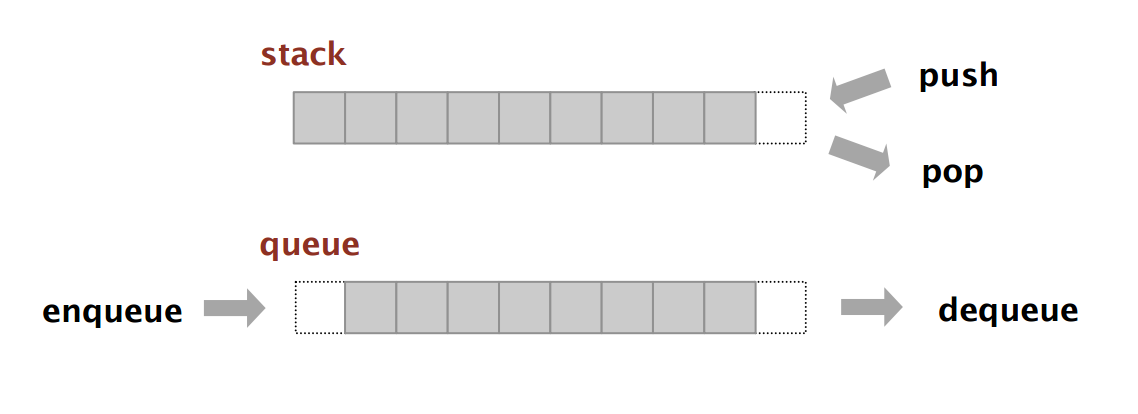
\includegraphics[scale=0.46]{stack_queue.png}
\end{center}

\textbf{Дек (Deque = Double-ended queue)} - это АТД, который представляет собой коллекцию элементов, менять которые можно только с помощью четырёх операций:
\begin{itemize}
\item \textbf{push\_back} - добавить элемент в конец.
\item \textbf{push\_front} - добавить элемент в начало.
\item \textbf{pop\_back} - извлечь элемент с конца.
\item \textbf{pop\_front} - извлечь элемент с начала.\\
\end{itemize}

\textbf{Очередь с приоритетом (Priority Queue)} - это АТД, который представляет собой коллекцию элементов, менять которые можно только с помощью двух операций:
\begin{itemize}
\item \textbf{insert} - добавить элемент.
\item \textbf{extract\_best} - извлечь из очереди элемент с наибольшим приоритетом. 
\end{itemize}
То, что будет являться приоритетом может различаться. Это может быть как сам элемент, часть элемента (например, одно из полей структуры) или другие данные, подаваемые на вход операции \textbf{insert} вместе с элементом. В простейшем случае, приоритетом является сам элемент (тогда очередь с приоритетом просто возвращает максимальный элемент) или сам элемент со знаком минус (тогда очередь с приоритетом возвращает минимальный элемент).


\subsection*{Реалицация очереди с приоритетом на основе массива.}
\begin{lstlisting}
#include <stdio.h>
#include <stdlib.h>
#define MAX_SIZE 1000

struct priority_queue {
	int data[MAX_SIZE];
	int size;
};
typedef struct priority_queue PriorityQueue;

void init(PriorityQueue* pq) {
	pq->size = 0;
}
void insert(PriorityQueue* pq, int x) {
	if (pq->size == MAX_SIZE) {
		printf("Error! Can't insert into the priority queue\n");
		exit(1);
	}
	pq->data[pq->size] = x;
	pq->size++;
}
int extract(PriorityQueue* pq) {
	if (pq->size == 0) {
		printf("Error! Can't extract from the priority queue\n");
		exit(1);
	}
	// Находим минимальный элемент
	int min_index = 0;
	for (int i = 1; i < pq->size; i++)
		if (pq->data[i] < pq->data[min_index])
			min_index = i;
	int result = pq->data[min_index];
	
	// Сдвигаем элементы на 1 влево
	for (int i = min_index + 1; i < pq->size; i++)
		pq->data[i-1] = pq->data[i];
	pq->size--;
	
	return result;
}
int main() {
	PriorityQueue a;
	init(&a);
	int numbers[] = {54, 32, 12, 16, 42, 53, 26, 91, 21, 43, 64, 75, 64, 37, 45};
	for (int i = 0; i < 15; i++)
		insert(&a, numbers[i]);
	
	for (int i = 0; i < 15; i++) {
		printf("%d ", extract(&a));
	}
}
\end{lstlisting}
Данная реализация очереди с приоритетом имеет один очень большой недостаток - операция извлечения \textbf{extract} очень неэффективна. Алгоритмическая сложность данной операции равна $O(N)$. Т.е. количество действий, необходимых чтобы совершить один \textbf{extract} зависит от $N$ следующим образом: $K \approx cN$, где $N$ - количество элементов в очереди, $c$ - некоторая константа.


\end{document}